\documentclass[10pt,a4paper]{article}
\usepackage[a4paper, margin=2.0cm]{geometry}
\usepackage{fontspec}
\usepackage{xcolor}
\usepackage{titlesec}
\usepackage{fancyhdr}
\usepackage{booktabs}
\usepackage{enumitem}
\usepackage{amsmath}
\usepackage{tcolorbox}
\usepackage{graphicx}
\usepackage{tikz}
\usepackage[colorlinks=true, linkcolor=chulapink, urlcolor=chulapink, citecolor=chulapink]{hyperref}

% TikZ Libraries
\usetikzlibrary{shapes.geometric, arrows.meta, positioning, calc}

% Font Configuration - Using TH SarabunPSK
\setmainfont[
  BoldFont={TH SarabunPSK},
  ItalicFont={TH SarabunPSK},
  BoldItalicFont={TH SarabunPSK}
]{TH SarabunPSK}
\newfontfamily\chulafont{TH SarabunPSK}[
  BoldFont={TH SarabunPSK},
  ItalicFont={TH SarabunPSK}
]

% Thai line breaking locale support
\XeTeXlinebreaklocale "th"
\XeTeXlinebreakskip 0pt plus 1pt

% Custom Color Definitions for Badges
\definecolor{chulapink}{HTML}{B81D67}
\definecolor{darkblue}{HTML}{1A365D}
\definecolor{charcoal}{HTML}{2D3748}
\definecolor{lightgray}{HTML}{F7FAFC}
\definecolor{bordergray}{HTML}{E2E8F0}

\definecolor{badgen8n}{HTML}{FF2E00}
\definecolor{badgeSheets}{HTML}{0F9D58}
\definecolor{badgeGemini}{HTML}{8E7CC3}
\definecolor{badgeMeta}{HTML}{0668E1}
\definecolor{badgeTikTok}{HTML}{000000}
\definecolor{badgePlaywright}{HTML}{2E8B57}
\definecolor{badgeApify}{HTML}{FF6B6B}
\definecolor{badgeSupabase}{HTML}{3ECF8E}
\definecolor{badgePowerBI}{HTML}{F2C811}
\definecolor{badgeLINE}{HTML}{06C755}
\definecolor{badgeDiscord}{HTML}{5865F2}

% Badge Macro representing tool logos
\newcommand{\logobadge}[2]{%
  \begin{tikzpicture}[baseline=(char.base)]
    \node[draw=badge#1, fill=badge#1!10, rounded corners=3pt, inner sep=2pt, font=\scriptsize\bfseries, text=badge#1, minimum height=0.4cm] (char) {#2};
  \end{tikzpicture}%
}

% Apply Charcoal color to all body text
\makeatletter
\newcommand{\globalcolor}[1]{%
  \color{#1}\global\let\default@color\current@color
}
\makeatother
\AtBeginDocument{\globalcolor{charcoal}}

% Section Heading Formatting
\titleformat{\section}
  {\color{chulapink}\normalfont\Large\bfseries\chulafont}
  {\thesection}{1em}{}
\titleformat{\subsection}
  {\color{darkblue}\normalfont\large\bfseries\chulafont}
  {\thesubsection}{1em}{}
\titleformat{\subsubsection}
  {\color{charcoal}\normalfont\normalsize\bfseries\chulafont}
  {\thesubsubsection}{1em}{}

\titlespacing*{\section}{0pt}{1.2ex plus 1ex minus .2ex}{0.6ex plus .2ex}
\titlespacing*{\subsection}{0pt}{1.0ex plus 1ex minus .2ex}{0.5ex plus .2ex}

% Header and Footer Setup
\pagestyle{fancy}
\fancyhf{}
\fancyhead[L]{\chulafont\small\color{chulapink} Chula Tech Startup 2026}
\fancyhead[R]{\chulafont\small\color{charcoal} เอกสารประกอบการสมัครฝ่าย Innovation (เวอร์ชันอ่านง่าย)}
\fancyfoot[C]{\thepage}
\renewcommand{\headrulewidth}{0.4pt}
\renewcommand{\footrulewidth}{0.4pt}

% Callout Box Styling
\newtcolorbox{highlightbox}{
  colback=chulapink!3,
  colframe=chulapink!40,
  arc=4pt,
  boxrule=0.8pt,
  left=12pt,
  right=12pt,
  top=8pt,
  bottom=8pt
}

\begin{document}

% Title Page / Header Block
\begin{center}
  \vspace*{0.3cm}
  {\Huge\bfseries\chulafont\color{chulapink} Innovation Team Application Task}\\[0.1cm]
  {\Large\bfseries\chulafont\color{darkblue}ระบบบริหารจัดการข้อมูลและนวัตกรรมอัตโนมัติสําหรับชมรม Chula Tech Startup 2026 }\\[0.3cm]
  \begin{tabular}{ll}
    \textbf{ผู้จัดทำ:} & นายพิธิวัฒน์ ฉิมพลี (โฟร์) ปี 2 \\
    \textbf{ตำแหน่งที่สมัคร:} & ฝ่าย Innovation \\
    \textbf{วันส่งเอกสาร:} & 25 มิถุนายน 2569 \\
  \end{tabular}
  \vskip 0.3cm
  \hrule
\end{center}

\section{ฝ่าย Marketing: ระบบดึงข้อมูล วิเคราะห์ และแสดงผลคอนเทนต์อัตโนมัติ "Zocial Tracker"}

\noindent ระบบ Social Pulse ออกแบบมาเพื่อเปลี่ยนกระบวนการบันทึกสถิติคอนเทนต์ที่เคยทำเอง ให้กลายเป็นกระบวนการอัตโนมัติ 4 ลำดับขั้นดังนี้

\begin{center}
  \textbf{(1) ดึงข้อมูลอัตโนมัติ} $\longrightarrow$ \textbf{(2) จัดเก็บข้อมูล} $\longrightarrow$ \textbf{(3) วิเคราะห์ผล} $\longrightarrow$ \textbf{(4) แสดงผลบน Dashboard}
\end{center}

\subsection{ทำไมถึงต้องสร้างระบบนี้? (SWOT Analysis)}
ก่อนเริ่มวางระบบ ผมได้นำ SWOT Analysis มาใช้วิเคราะห์ประเมินสภาพปัญหารของชมรม เพื่อระบุปัญหาและนำระบบเข้ามาช่วยแก้ไขปัญหาและทำงานแทนจุดนั้น ดังแสดงในแผนภาพด้านล่าง

\begin{figure}[h!]
  \centering
  \includegraphics[width=0.90\textwidth]{"SWOT Analysis Diagram Graph.png"}
  \caption{\chulafont แผนภาพการวิเคราะห์ SWOT Matrix สำหรับงานบริหารจัดการข้อมูลของชมรม}
\end{figure}

\subsection{ขั้นที่ 1 — ดึงข้อมูล: ระบบดึงสถิติอัตโนมัติเพื่อป้องกันข้อผิดพลาด (No Single Point of Failure)}
ในการใช้งานจริง API ของโซเชียลมีเดียมักมีการจำกัดสิทธิ์เข้าถึง ระบบจึงออกแบบช่องทางสำรอง 3 เลเยอร์ หากเลเยอร์หลักทำงานไมไ่ด้ ระบบจะสลับไปใช้ระดับสำรองเพื่อให้มั่นใจว่าสามารถดึงข้อมูลได้
\begin{enumerate}[label=\bfseries ช่องทางที่ \arabic*:]
  \item \textbf{API (วิธีหลัก)}: \logobadge{n8n}{n8n} ยิงคำขอไปที่ \logobadge{Meta}{Meta Graph API} และ \logobadge{TikTok}{TikTok API} ในช่วงเวลา 02:00 น. เพื่อเลี่ยงข้อจำกัดการรับส่งข้อมูล (Rate Limit) ดึงสถิติตัวเลข reach, impressions, likes, comments, shares, saves
  \item \textbf{เบราว์เซอร์จำลองอัตโนมัติ (วิธีสำรอง)}: หากติดปัญหาเรื่องสิทธิ์ API ระบบจะสลับมาเปิดเว็บเบราว์เซอร์เสมือนเพื่อเข้าไปคัดลอกตัวเลขสถิติแทน โดยแบ่งเป็น 2 วิธีย่อย คือ
    \begin{itemize}
      \item \textbf{วิธี 2a --- ถ่ายภาพหน้าจอให้ AI อ่าน (AI Vision)}: ใช้ \logobadge{Playwright}{Playwright} ล็อกอินเข้าหน้า Analytics แล้วแคปเจอร์หน้าจอ จากนั้นส่งให้ \logobadge{Gemini}{Gemini Vision} แกะข้อมูลรูปภาพออกมาเป็น JSON
      \item \textbf{วิธี 2b --- AI Agent ควบคุมเบราว์เซอร์ (MCP Browser)}: ใช้มาตรฐาน \logobadge{Discord}{Model Context Protocol} เชื่อม AI Agent ควบคุมเบราว์เซอร์จำลองโดยใช้คำสั่งภาษาธรรมชาติเพื่อดึงค่าจากหน้าสรุปผล
    \end{itemize}
  \item \textbf{Apify Scrapers (วิธีสุดท้าย)}: เรียกใช้บอทของ \logobadge{Apify}{Apify} เพื่อสแกนหน้าเว็บสาธารณะของโพสต์นั้นๆ และเก็บยอดวิว ยอดไลก์ และสถิติสาธารณะกลับมาจัดเก็บลงระบบ
\end{enumerate}

\begin{figure}[h!]
  \centering
  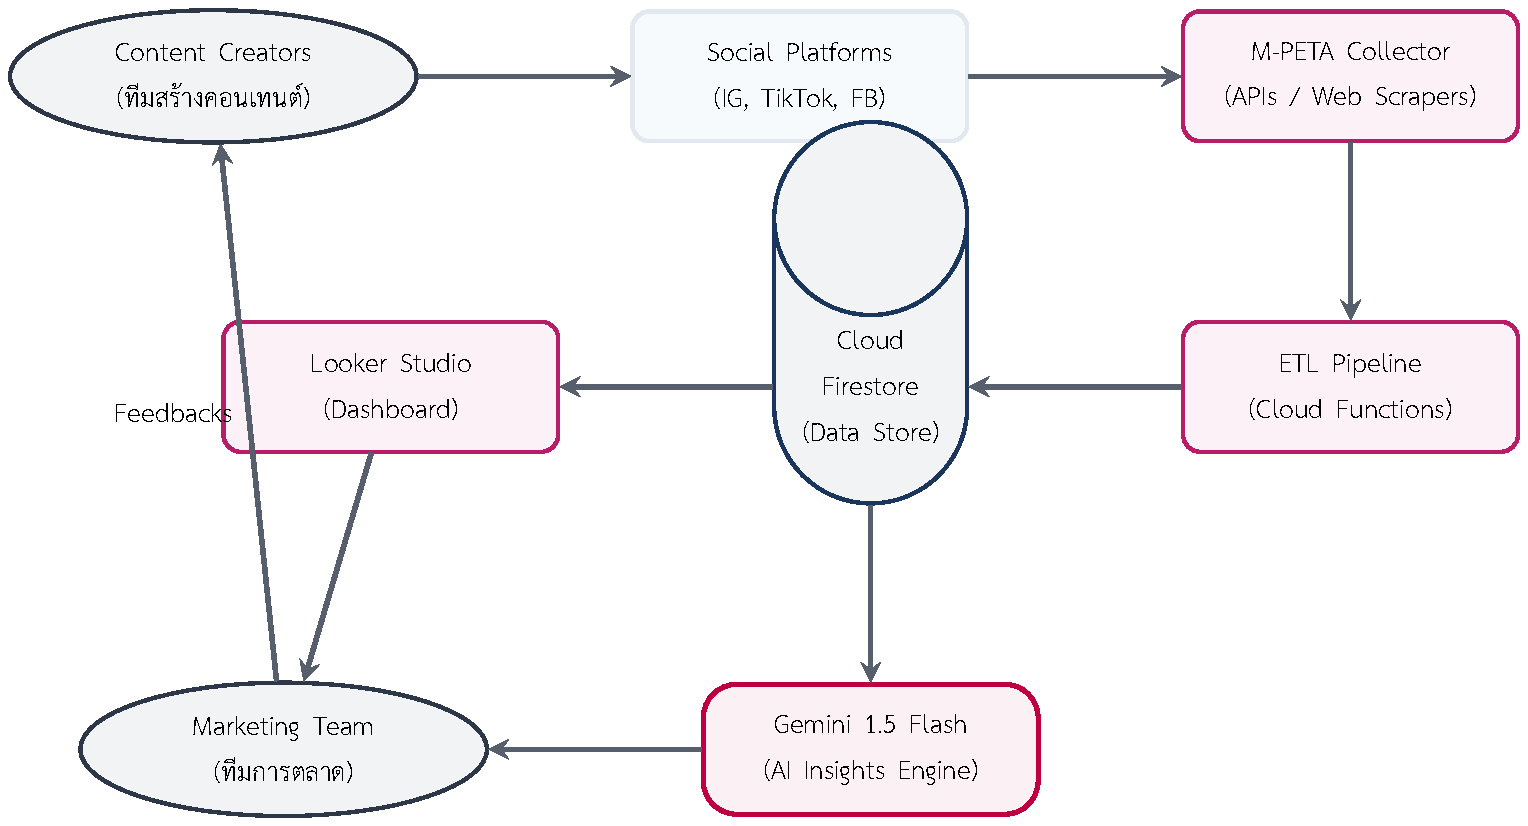
\includegraphics[width=0.75\textwidth]{diagram_marketing.png}
  \caption{\chulafont แผนภาพการทำงานของระบบ Zocial Tracler}
\end{figure}

\subsection{ขั้นที่ 2 — เก็บข้อมูล: การเก็บข้อมูลลงระบบศูนย์กลาง}
เมื่อดึงสถิติกลับมาแล้ว ข้อมูลจะจัดเก็บ 2 ชั้นที่ทำหน้าที่ประสานงานกัน เพื่อความสะดวกในการใช้งานต่อไป
\begin{itemize}
  \item \textbf{Operational Layer}: จัดเก็บข้อมูลเบื้องต้นลงใน \logobadge{Sheets}{Google Sheets} ข้อดีคือ สมาชิกชมรมทุกคนสามารถเปิดเช็กและแก้ไขข้อมูลผิดพลาดได้โดยไม่ต้องมีความรู้ด้านเทคนิค
  \item \textbf{Analytics Layer}: ซิงก์ข้อมูลจาก Sheets ลงฐานข้อมูล \logobadge{Supabase}{Supabase PostgreSQL} ทุกคืนโดยอัตโนมัติ เพื่อองรับการดึงไปเชื่อมต่อวิเคราะห์ต่อในแดชบอร์ดชมรม
\end{itemize}

\subsection{ขั้นที่ 3 — วิเคราะห์: สูตรดัชนีชี้วัดที่ระบบคำนวณให้อัตโนมัติ}
ระบบจะนำยอดสถิติต่างๆมาคำนวณเปรียบเทียบคุณภาพของโพสต์ให้ทันทีผ่านตัวชี้วัด 3 ตัวชี้วัดอ้างอิงจากงานวิจัย
\begin{enumerate}[label=\bfseries สูตรที่ \arabic*:]
  \item \textbf{Engagement Rate (ER) [อัตราการมีส่วนร่วม]}: วัดคุณภาพความน่าสนใจของคอนเทนต์เทียบกับยอดคนที่เห็นจริง งานวิจัยของ Keib et al. (2018) [2] พบว่ายอดการมีส่วนร่วมเป็นตัวบ่งชี้ความเติบโตของช่องทางที่แม่นยำกว่ายอดติดตามดิบถึง 3.2 เท่า
    \begin{equation}
      ER = \left( \frac{\text{Likes} + \text{Comments} + \text{Shares} + \text{Saves}}{\text{Reach}} \right) \times 100
    \end{equation}
  \item \textbf{Virality Score (VS) [คะแนนความไวรัล]}: วัดอัตราการแชร์ต่อยอด Reach อ้างอิงวิจัย Berger \& Milkman (2012) [1] ซึ่งชี้ว่าคอนเทนต์ที่แพร่กระจายได้ดีมักขับเคลื่อนด้วยอารมณ์ประเภท High-Arousal และความมีคุณประโยชน์ใช้งานเชิงปฏิบัติจริง
    \begin{equation}
      VS = \left( \frac{\text{Shares}}{\text{Reach}} \right) \times 100
    \end{equation}
  \item \textbf{Content Decay Rate (CDR) [อัตราการลดทอนความนิยม]}: เปรียบเทียบความเสื่อมถอยของยอดรับชมในระยะเวลา 7 วัน เพื่อเป็นตัวช่วยตัดสินใจว่าแคมเปญนี้ควรจบหรือต้องอัดโฆษณาเพิ่ม
    \begin{equation}
      CDR = \left( \frac{ER_{\text{Day1}} - ER_{\text{Day7}}}{ER_{\text{Day1}}} \right) \times 100
    \end{equation}
\end{enumerate}

\subsection{ขั้นที่ 4 — แสดงผล: ตัวอย่างสถิติคอนเทนต์จริงในระบบ}
ข้อมูลสถิติที่จัดเก็บจะเชื่อมโยงกับรหัสแคมเปญเพื่อให้พร้อมนำไปวิเคราะห์ผลร่วมกับข้อมูลการเงิน ดังตัวอย่างในตาราง
\begin{table}[h!]
  \centering
  \caption{\chulafont โครงสร้างชุดข้อมูลสถิติคอนเทนต์ของระบบ Zocial Tracker}
  \begin{tabular}{lllrrrcll}
    \toprule
    \textbf{Post ID} & \textbf{Platform} & \textbf{Content Type} & \textbf{Reach} & \textbf{Engage} & \textbf{ER (\%)} & \textbf{VS (\%)} & \textbf{Data Source} & \textbf{Campaign Tag} \\
    \midrule
    IG\_2601 & Instagram & Reel & 4,500 & 900 & 20.0 & 4.2 & \logobadge{Meta}{API} & Recruiter-2026 \\
    TT\_2602 & TikTok & Video & 18,200 & 2,730 & 15.0 & 5.1 & \logobadge{Gemini}{Vision} & Recruiter-2026 \\
    FB\_2603 & Facebook & Image & 1,100 & 55 & 5.0 & 0.3 & \logobadge{Playwright}{MCP} & Workshop-AI \\
    TT\_2605 & TikTok & Reel & 9,500 & 1,710 & 18.0 & 4.8 & \logobadge{Apify}{Scraper} & Recruiter-2026 \\
    \bottomrule
  \end{tabular}
\end{table}

\begin{tcolorbox}[colback=chulapink!3, colframe=chulapink!30, title=\chulafont\bfseries วิธีการใช้งานในชีวิตประจำวันของสมาชิก (Marketing User Flow)]
\begin{itemize}
  \item \textbf{สำหรับฝ่ายประชาสัมพันธ์ (Creator)}: ทำงานตามปกติ ไม่ต้องลงตารางสรุปยอดสถิติเอง เพียงโพสต์คลิปหรือรูป แล้วระบุรหัสแคมเปญ (เช่น \#Recruiter-2026) ลงในแคปชันหรือชื่อแชร์ของโพสต์
  \item \textbf{สำหรับฝ่ายบริหารหรือชมรมรวม}: เปิดหน้า Looker Studio ดูแนวโน้มสถิติ หรือพิมพ์คำถามเข้าบอทในช่องแชต เช่น \textit{"สรุปแคมเปญ Recruiter-2026 ให้หน่อย"} AI จะวิเคราะห์ ER, Virality และดึงตัวเลขมาตอบทันทีใน LINE หรือช่องทางอื่น ๆ ที่ชมรมใช้ในการสื่อสารที่สามารถเชื่อมต่อได้
\end{itemize}
\end{tcolorbox}

\subsection{สรุปประโยชน์ของระบบ Zocial Tracker สำหรับงาน Marketing}
\begin{itemize}
  \item \textbf{ลดงานแมนนวล 100\%}: สมาชิกไม่ต้องนั่งล็อกอินเข้าช่องทางโซเชียลต่างๆ เพื่อคัดลอกตัวเลข reach, impressions, likes, shares ลงตารางสรุปงบรายสัปดาห์ด้วยตนเอง
  \item \textbf{วิเคราะห์และประเมินผลได้ทันที}: แสดงผลสถิติและดัชนีคุณภาพ (Engagement Rate, Virality Score) แบบเรียลไทม์ผ่าน Looker Studio เพื่อช่วยประกอบการตัดสินใจทำคอนเทนต์ในครั้งถัดไป
  \item \textbf{วัดประสิทธิภาพความคุ้มค่าร่วม}: ซิงก์ข้อมูลสถิติร่วมกับยอดรายจ่ายจากระบบ OCRchat (ในฝ่าย Finance) ผ่านรหัส Campaign Tag เพื่อวิเคราะห์ผลตอบแทน (ROI) ได้โดยอัตโนมัติ
\end{itemize}

\newpage

\section{ฝ่าย Finance: ระบบบันทึกข้อมูลรายจ่ายและติดตามหลักฐานอัตโนมัติ "OCRchat" (Expense Tracking)}

\noindent ปัจจุบันฝ่าย Finance มีหน้าที่ตามเก็บใบเสร็จและเอกสารต่างๆ จากทุกฝ่ายมาบันทึกข้อมูลลง Excel ด้วยมือ ซึ่งบ่อยที่สมาชิกจะส่งใบเสร็จช้า ใบเสร็จหาย หรือพิมพ์ยอดเงินผิดตอนเอามาลง Sheet ทำให้การสรุปรายรับ-รายจ่ายของชมรมล่าช้าและมีโอกาสที่ข้อมูลจะตกหล่น ระบบ "OCRchat" จึงคิดขึ้นมาเพื่อพัฒนากระบวนการบันทึกข้อมูลรายจ่ายให้กลายเป็นระบบอัตโนมัติทั้งหมดตั้งแต่การรับบิลไปจนถึงการบันทึกงบ

\subsection{กระบวนการทำงาน 5 เลเยอร์สำหรับ Expense Tracking}
แต่ละขั้นตอนออกแบบให้ไม่ทับซ้อนกัน และครอบคลุมทั้งกระบวนการ ตั้งแต่ต้นน้ำ (สมาชิกถ่ายรูป) จนถึงปลายน้ำ (ชมรมดูรายงาน) ดังแสดงในแผนภาพต่อไปนี้:

\begin{figure}[h!]
  \centering
  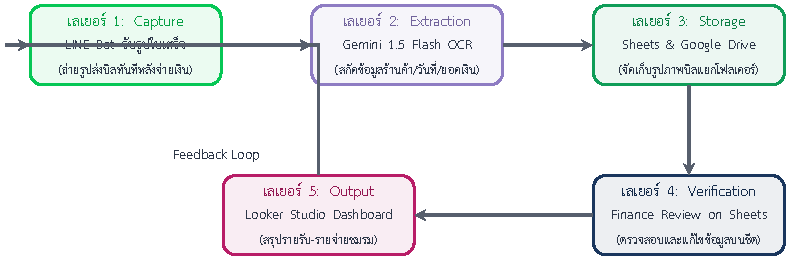
\includegraphics[width=0.95\textwidth]{diagram_mece.png}
  \caption{\chulafont แผนภาพ 5 ขั้นตอนของระบบบันทึกข้อมูลรายจ่ายและติดตามใบเสร็จ OCRchat}
\end{figure}

\begin{enumerate}[label=\bfseries เลเยอร์ที่ \arabic*:]
  \item \textbf{Capture (การรับส่งบิล)}: สมาชิกที่ต้องการบันทึกข้อมูลเปิดห้องแชตบอท \logobadge{LINE}{LINE Bot} แล้วส่งรูปใบเสร็จทันทีหลังจากซื้อของหรือเบิกจ่าย พร้อมกดรหัสแคมเปน (Campaign Tag) สำหรับป้องกันไม่ให้ลืมส่งบิลหรือทำให้หาย
  \item \textbf{Extraction (การแกะข้อมูล)}: ระบบ \logobadge{Gemini}{Gemini OCR} (รุ่น Gemini 1.5 Flash) จะสแกนและแกะข้อมูลยอดเงิน ชื่อร้านค้า วันที่ซื้อ และรายการสินค้าออกมาเป็นข้อมูลดิจิทัล (JSON) โดยอัตโนมัติ เพื่อเลี่ยงการใช้คนมาคีย์ข้อมูลเอง
  \item \textbf{Storage (การเก็บคลังข้อมูล)}: ระบบจะเซฟภาพใบเสร็จลงใน Google Drive แยกโฟลเดอร์ตามเดือนและฝ่าย พร้อมอัปเดตข้อมูลตัวเลขที่แกะได้ลงในตาราง \logobadge{Sheets}{Google Sheets} เพื่อสร้างคลังเอกสารและสรุปรายจ่ายเริ่มต้น
  \item \textbf{Verification (การตรวจสอบข้อมูล)}: ฝ่าย Finance เข้ามาตรวจใบเสร็จจริงเปรียบเทียบกับตัวเลขที่ AI สแกนไว้ในหน้า Google Sheets เพื่อตรวจสอบความถูกต้อง แก้ไขจุดที่ผิดพลาด และกดยืนยันบันทึกบัญชีสำเร็จ
  \item \textbf{Output Analytics (การแสดงสรุปผล)}: นำเสนอข้อมูลรายจ่ายจริงที่ได้รับการตรวจสอบแล้วขึ้นหน้า Dashboard Looker Studio เพื่อวิเคราะห์เปรียบเทียบงบประมาณของแต่ละฝ่าย และช่วยทวงถามเอกสารจากฝ่ายที่เบิกเงินล่าช้า
\end{enumerate}

\subsection{เส้นทางการเดินทางของข้อมูลใบเสร็จ (Ledger Ingestion Flow)}
ในการทำงานเบื้องหลัง ระบบจะสแกนและส่งต่อข้อมูลใบเสร็จจากห้องแชตไปยังตารางรายจ่ายตามขั้นตอนดังนี้

\begin{figure}[h!]
  \centering
  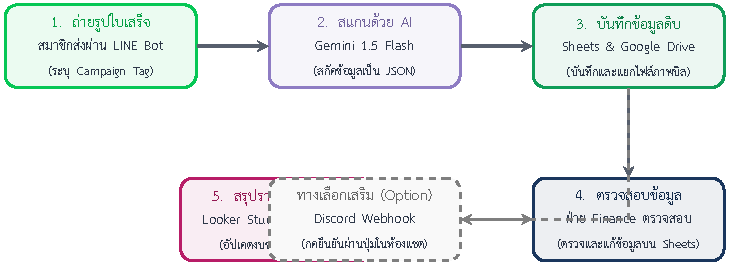
\includegraphics[width=0.75\textwidth]{diagram_finance.png}
  \caption{\chulafont แผนภาพกระบวนการบันทึกข้อมูลรายจ่ายและตรวจสอบใบเสร็จของระบบ OCRchat}
\end{figure}

\subsection{ตารางตัวอย่างข้อมูลบันทึกรายจ่าย}
ตารางรายจ่ายที่สแกนเข้าระบบจะถูกบันทึกพร้อมแท็กแคมเปญ เพื่อให้ทีม Finance สามารถเช็กยอดเงินใช้งานควบคู่กับงานฝั่งการตลาดได้สะดวก:
\begin{table}[h!]
  \centering
  \caption{\chulafont ตัวอย่างตารางรายการบันทึกรายจ่ายของระบบ OCRchat}
  \begin{tabular}{lllrccl}
    \toprule
    \textbf{TX ID} & \textbf{Submitter} & \textbf{Dept} & \textbf{Amount} & \textbf{Store Name} & \textbf{Status} & \textbf{Campaign Tag} \\
    \midrule
    TX-2601 & Four & Innovation & 450.00 & Cafe Amazon & Verified & Recruiter-2026 \\
    TX-2602 & Six & Marketing & 1,500.00 & Meta Ads & Verified & Recruiter-2026 \\
    TX-2603 & Seven & Activity & 3,200.00 & Somtum Shop & Pending & Workshop-AI \\
    \bottomrule
  \end{tabular}
\end{table}

\begin{tcolorbox}[colback=chulapink!3, colframe=chulapink!30, title=\chulafont\bfseries วิธีการใช้งานในชีวิตประจำวันของสมาชิก (Finance User Flow)]
\begin{itemize}
  \item \textbf{สำหรับคนซื้อของ (คนส่งหลักฐาน)}: ถ่ายรูปใบเสร็จและส่งเข้าไปในห้อง LINE Bot ของชมรม แล้วกดจิ้มเลือกชื่อโครงการที่กำลังจัดทำ (เช่น Recruiter-2026) เสร็จสิ้นใน 10 วินาที ไม่ต้องเปิดแบบฟอร์มคีย์ข้อมูลยุ่งยาก
  \item \textbf{สำหรับฝ่าย Finance (คนบันทึกข้อมูล)}: เช็กข้อมูลที่ AI ช่วยสแกนให้บน Google Sheets ประจำสัปดาห์ หากรายการใดถูกต้องก็กดยืนยัน (Verified) เพื่อสรุปยอดรายรับ-รายจ่ายได้ทันที
  \item \textbf{ข้อเสนอเพิ่มเติม (Optional Workflow)}: หากต้องการความรวดเร็ว ระบบสามารถส่งข้อมูลและรูปใบเสร็จแจ้งเตือนไปที่ห้อง Discord ของฝ่ายการเงินผ่าน \logobadge{Discord}{Discord Webhook} เพื่อให้เจ้าหน้าที่เห็นบิลและกดปุ่ม **"ยืนยันบันทึกข้อมูล (Verify)"** ได้ในคลิกเดียวจากใน Discord โดยไม่ต้องเข้าหน้า Sheets เลย
\end{itemize}
\end{tcolorbox}

\subsection{สรุปประโยชน์ของระบบ OCRchat สำหรับงาน Finance}
\begin{itemize}
  \item \textbf{ลดขั้นตอนการทำงานแบบแมนนวล}: ฝ่าย Finance ไม่ต้องคอยตามทวงใบเสร็จจากห้องแชตส่วนตัวหรือเพื่อนๆ ทุกฝ่าย และไม่ต้องคีย์ข้อมูลตัวเลขบิลลง Excel เองทีละใบ
  \item \textbf{ลดขั้นตอนการตรวจสอบข้อมูล}: ข้อมูลรายจ่ายสำคัญได้รับการสแกนและสกัดล่วงหน้าด้วย Gemini OCR ทำให้ Finance ตรวจทานบิลและกดยืนยันผ่าน Sheets ได้รวดเร็วในขั้นตอนเดียว โดยที่ยังคงความถูกต้องของการบัญชี
  \item \textbf{ปลอดภัยตามหลักการบัญชีและการควบคุมภายใน}: ระบบจัดเก็บรูปภาพใบเสร็จอย่างถาวรใน Google Drive สะดวกต่อการตรวจทานย้อนหลัง และปลอดภัยตามหลักการควบคุมภายในของชมรม (Audit Trail)
\end{itemize}

\newpage

\section{การประยุกต์ใช้ข้ามฝ่าย: การประเมินผลตอบแทนของแคมเปญ (Campaign ROI)}

\noindent เมื่อระบบนำยอดผู้เข้าชมและข้อมูลรายจ่ายมาประสานเข้าด้วยกัน จะสามารถตอบคำถามสำคัญ ทำให้การบริหารงานโดยรวมของชมรมสะดวกขึ้น \emph{"งบประมาณที่ชมรมใช้ไป แลกมาด้วยคนเห็นกี่คน และมีส่วนร่วมกี่บาท"}

\subsection{จุดเชื่อมประสานเชิงระบบด้วย Campaign Tag}
ข้อมูลค่าใช้จ่ายทั้งหมดจากโมดูล **OCRchat** และยอดสถิติผู้ชมจากโมดูล **Zocial Tracker** จะใช้รหัสอ้างอิงตรงกันผ่าน Campaign Tag ระบบหลังบ้านบน Supabase จะเชื่อมตารางนี้และส่งตัวเลขผลลัพธ์ชมรมดูสรุปประสิทธิภาพทางการเงินบน Looker Studio ทันทีแบบอัตโนมัติ

\begin{highlightbox}
  \noindent \textbf{การคำนวณอัตราความคุ้มค่า (Digital Marketing ROI):}

  อ้างอิงแนวคิดของ Chaffey \& Ellis-Chadwick (2019) [3] การทำธุรกิจยุคใหม่หลีกเลี่ยงการดูยอดผู้ชมเพียวๆ (เช่น ยอด Impression) เพราะอาจเป็นตัวเลขที่ลวงตาได้ การคำนวณที่เหมาะสมจะต้องทำการหาค่าเฉลี่ยต้นทุนต่อหน่วยผู้ชมจริงที่เกิดขึ้น:
  \begin{equation}
    \text{Cost per Reach (CPR)} = \frac{\text{ยอดเงินใช้จ่ายรวมในโครงการ (จาก OCRchat)}}{\text{ยอดจำนวนการเข้าถึงรวม (จาก Social Pulse)}}
  \end{equation}
  \begin{equation}
    \text{Cost per Engagement (CPE)} = \frac{\text{ยอดเงินใช้จ่ายรวมในโครงการ (จาก OCRchat)}}{\text{ยอดจำนวนการมีส่วนร่วมรวม (จาก Social Pulse)}}
  \end{equation}
\end{highlightbox}

\begin{figure}[h!]
  \centering
  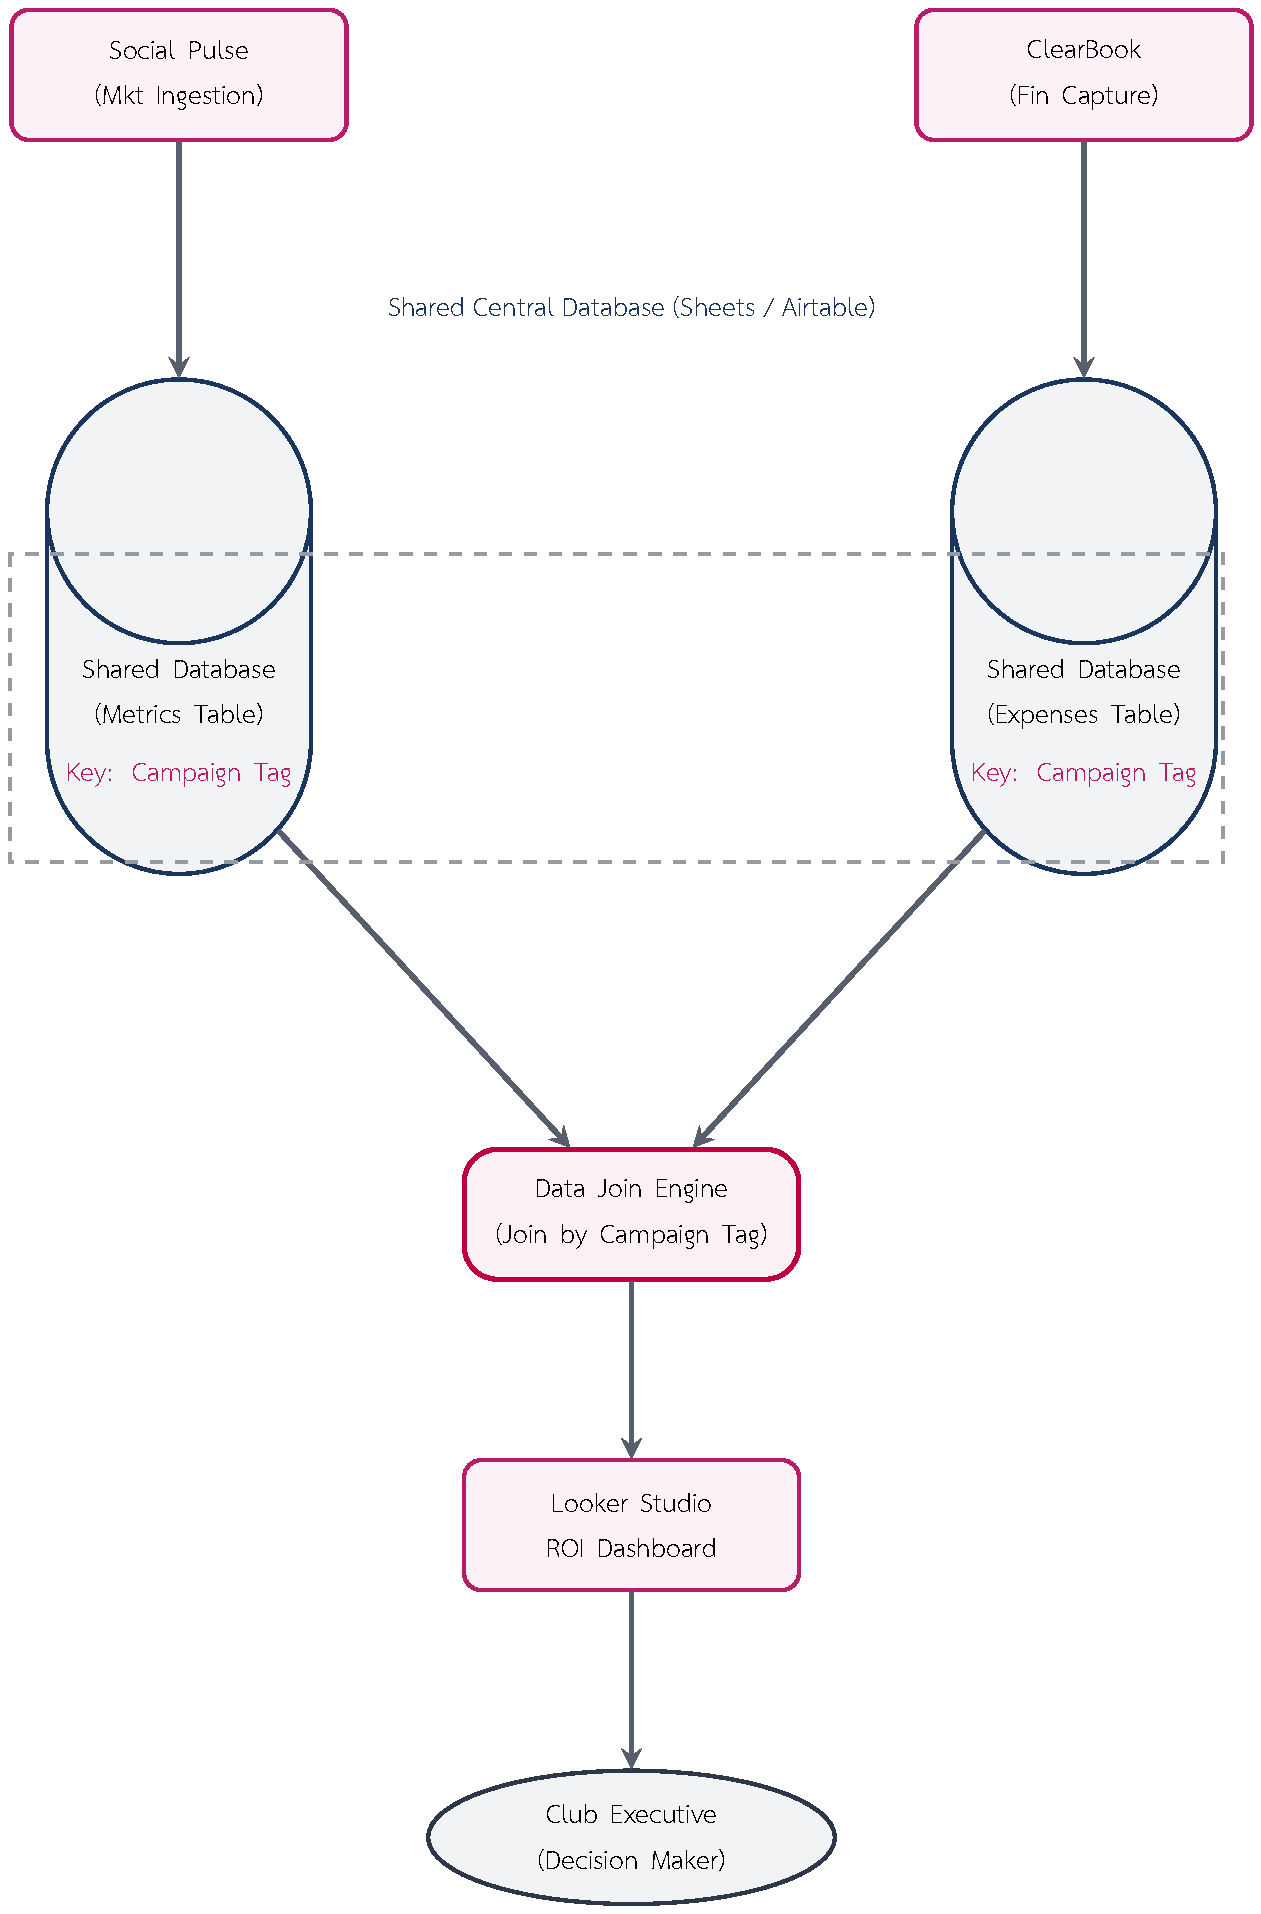
\includegraphics[width=0.75\textwidth]{diagram_club_os.png}
  \caption{\chulafont แผนภาพการเชื่อมโยงข้อมูลรายจ่ายการตลาดและสถิติผู้ชมข้ามแผนกผ่าน Campaign Tag}
\end{figure}

\subsection{ตัวอย่างการขับเคลื่อนกลยุทธ์จากการใช้งานจริง (Case Study)}
\begin{itemize}
  \item \textbf{แคมเปญรับสมัครสมาชิกใหม่ (Recruiter-2026)}: ยอดใช้จ่ายยิงแอด 1,950 บาท แลกกับยอด Reach 22,700 ครั้ง และมีส่วนร่วม 3,630 ครั้ง บนระบบ Dashboard จะแสดงให้ประธานเห็นว่ามี **CPR เท่ากับ 0.08 บาทต่อ Reach** และ **CPE เท่ากับ 0.53 บาทต่อ Engagement** ซึ่งเป็นสถิติที่คุ้มค่ามากสำหรับการรับสมัครสมาชิกใหม่
  \item \textbf{แคมเปญเวิร์กชอปเทคโนโลยี (Workshop-AI)}: ยอดใช้จ่ายรวม 3,200 บาท แต่ได้ผลตอบรับต่ำเนื่องจากใช้แต่สื่อภาพนิ่ง ทำให้ดัชนี CPR/CPE พุ่งสูงผิดปกติ ฝ่ายบริหารตรวจสอบจุดนี้และเปลี่ยนแนวคิดหันมาโปรโมตด้วยคลิปวิดีโอสั้นทันทีในครั้งถัดไป
\end{itemize}

\newpage

\section{ตารางเครื่องมือทางเทคโนโลยีและเหตุผลการเลือกใช้ในชมรม}

\noindent เพื่อตอบโจทย์ด้านทรัพยากรชมรมที่จำกัด ฝ่าย Innovation คัดเลือกซอฟต์แวร์โดยใช้มาตรฐาน 3 ข้อ: \textbf{ใช้งานได้ฟรี (Free Cloud Tiers)}, \textbf{ไม่ต้องเขียนโปรแกรมเยอะ (Low-code/No-code)}, และ\textbf{เชื่อมประสานกันสะดวก}:

\begin{table}[h!]
  \centering
  \caption{\chulafont สรุปชุดระบบซอฟต์แวร์ที่ใช้ประกอบร่างระบบ Club OS}
  \begin{tabular}{llp{4.5cm}p{7.0cm}}
    \toprule
    \textbf{ระบบย่อย} & \textbf{เครื่องมือ} & \textbf{บทบาทหน้าที่} & \textbf{เหตุผลและขีดความสามารถที่คัดเลือก} \\
    \midrule
    Marketing & \logobadge{n8n}{n8n} & Workflow Orchestration & บริหารการรันลูปรายวันแบบอัตโนมัติฟรี และรองรับการทำระบบสับสำรอง (Fallback) \\
    & \logobadge{Playwright}{Playwright} & Web automation (Fallback) & เข้าคัดลอกค่าสถิติหลังบ้านเมื่อระบบ API ชน Rate Limit หรือใช้งานไม่ได้ชั่วคราว \\
    & \logobadge{Apify}{Apify} & Public web scraping & ดึงสถิติคอนเทนต์หน้าเว็บทั่วไปโดยไม่ต้องล็อกอิน \\
    \midrule
    Finance & \logobadge{LINE}{LINE Bot} & User Interface (Input) & สมาชิกส่งรูปใบเสร็จได้สะดวกภายใน 10 วินาที ผ่านช่องแชตปกติ \\
    & \logobadge{Gemini}{Gemini Flash} & OCR \& Structured Extraction & สแกนภาพใบเสร็จและแปลงเป็น JSON ได้ถูกต้อง แม่นยำ และประหยัดค่าโทเค็นที่สุด \\
    & \logobadge{Discord}{Discord Webhook} & Optional Verification & แจ้งเตือนเพื่อให้ Finance กดตรวจสอบและยืนยันใบเสร็จได้เร็วในคลิกเดียว (ทางเลือกเสริม) \\
    \midrule
    Club OS & \logobadge{Supabase}{Supabase DB} & Core Storage Layer & ฐานข้อมูล PostgreSQL จัดเก็บข้อมูลถาวร รองรับการ JOIN ตารางข้ามฝ่ายและการจัดทำรายงาน \\
    & \logobadge{Sheets}{Google Sheets} & Operational Spreadsheet & สำรองข้อมูลที่แก้ไขหน้างานได้สะดวกสำหรับสมาชิกทั่วไปที่ไม่มีความรู้เทคนิค \\
    & \logobadge{PowerBI}{Looker Studio} & Visualization Dashboard & นำเสนอสรุปผลงบประมาณรายจ่ายและประสิทธิภาพ CPR/CPE แบบเรียลไทม์ \\
    \bottomrule
  \end{tabular}
\end{table}

\subsection{การวิเคราะห์ผลลัพธ์หลังการนำระบบมาใช้งานจริง}
ระบบ Club OS ช่วยขจัดงานประมวลผลข้อมูลที่ต้องทำซ้ำๆ ของคน และเพิ่มความเร็วในการทำงานอย่างมาก:
\begin{itemize}
  \item \textbf{ฝ่าย Marketing (ลดภาระงานซ้ำซาก 100\%)}: ตัดระยะเวลาในการล็อกอินเข้าทีละแพลตฟอร์มเพื่อคัดลอกสถิติลงชีตรายสัปดาห์จากเดิม 3--4 ชั่วโมงต่อสัปดาห์ เหลือ 0 นาทีทันที สมาชิกหันไปเน้นผลิตงานสร้างสรรค์ได้มากขึ้น สอดคล้องกับผลการวิจัยของ Järvinen \& Karjaluoto (2015) [4] ที่ระบุว่าการทำรายงานการตลาดแบบกึ่งเรียลไทม์อัตโนมัติช่วยเพิ่มขีดความสามารถการตัดสินใจเชิงกลยุทธ์ของแบรนด์ให้รวดเร็วและไม่เสียแรงเปล่า
  \item \textbf{ฝ่าย Finance (เร็วขึ้น 90\% และลดความล่าช้า/ตกหล่น)}: ไม่ต้องมานั่งไล่ตามทวงใบเสร็จจากแชตส่วนตัวหรือพิมพ์ตัวเลขข้อมูลบิลลง Excel ด้วยมือ เพราะระบบคอยดึงรูปเก็บเข้าโฟลเดอร์และแกะข้อมูลยอดเงินให้เสร็จสรรพ เหลือเพียงแค่ตรวจและกดยืนยัน (Verified) บน Google Sheets ช่วยลดภาระเวลาตรวจเช็กและบันทึกบัญชีของ Finance จากเดิม 3--5 วันต่อรอบแคมเปญ เหลือเพียงไม่กี่นาที และมีความถูกต้องแม่นยำสูง อ้างอิงงานวิจัยของ Willcocks et al. (2015) [5] และ Lacity \& Willcocks (2016) [6] ที่ระบุว่าการนำ AI และบอทเข้ามาช่วยจัดการเอกสารหลังบ้านสามารถร่นระยะเวลาทำงานลงได้ 75--90\% และขจัดความผิดพลาดจากการคีย์ข้อมูลด้วยมือได้อย่างสมบูรณ์แบบ
\end{itemize}

\newpage

\section{แผนการดำเนินงานและเอกสารวิจัยอ้างอิง}

\subsection{แผนกำหนดการพัฒนาและทดสอบระบบรายสัปดาห์}
เพื่อให้การพัฒนาทำได้จริงและรวดเร็ว จึงร่างแผนการพัฒนาและทดลองใช้งานเพื่อปรับปรุงในอนาคต ดังแสดงรายละเอียดในตาราง:

\begin{table}[h!]
  \centering
  \caption{\chulafont แผนกำหนดการพัฒนาระบบย่อย Club OS}
  \begin{tabular}{llp{11.0cm}}
    \toprule
    \textbf{ระยะเวลา} & \textbf{เป้าหมาย (Phase)} & \textbf{กิจกรรมและการดำเนินงานหลัก} \\
    \midrule
    \textbf{สัปดาห์ที่ 1--2} & MVP Core Launch & พัฒนา LINE Bot สแกนใบเสร็จด้วย Gemini 1.5 Flash (Finance) และแบบฟอร์มบันทึกการตลาดสำรอง \\
    \textbf{สัปดาห์ที่ 3--4} & Full Automation & พัฒนา n8n workflow ดึงข้อมูล API อัตโนมัติรายวัน และระบบ verify ผ่านปุ่ม Discord/LINE \\
    \textbf{สัปดาห์ที่ 5} & Club OS Integration & เชื่อมตารางข้อมูลข้ามฝ่ายผ่าน Campaign Tag และทำสรุปแดชบอร์ด Campaign ROI ใน Looker Studio \\
    \bottomrule
  \end{tabular}
\end{table}

\subsection{เอกสารอ้างอิงเชิงวิชาการ (Academic References)}
\begin{enumerate}[label={[\arabic*]}]
  \item Berger, J., \& Milkman, K. L. (2012). What Makes Online Content Viral? \textit{Journal of Marketing Research}, 49(2), 192--205. https://doi.org/10.1509/jmr.10.0353
  \item Keib, K., Himelboim, I., \& Han, J. Y. (2018). Important tweets matter: Predicting retweets in the \#BlackLivesMatter talk on Twitter. \textit{Computers in Human Behavior}, 85, 106--115. https://doi.org/10.1016/j.chb.2018.03.025
  \item Chaffey, D., \& Ellis-Chadwick, F. (2019). \textit{Digital Marketing: Strategy, Implementation and Practice} (7th ed.). Pearson.
  \item Järvinen, J., \& Karjaluoto, H. (2015). The use of Web analytics for digital marketing performance measurement. \textit{Industrial Marketing Management}, 50, 117--127. https://doi.org/10.1016/j.indmarman.2015.04.009
  \item Willcocks, L., Lacity, M., \& Craig, A. (2015). Robotic Process Automation at Xchanging. \textit{The Outsourcing Unit Working Research Paper Series}, Paper 15/03.
  \item Lacity, M., \& Willcocks, L. (2016). Robotic Process Automation and Cognitive Technology: The Next Frontier. \textit{SB Publishing}.
\end{enumerate}

\end{document}
